\chapter{Figures}


\section{Figures}

\textit{\blindtext }
\newline

\begin{lstlisting}
\begin{figure}[htb]
    \centering
    
\includegraphics[width=0.65\textwidth]{images/a}
    \caption{Figure 1}
    \label{fig: 1}
\end{figure} 
\end{lstlisting}

\begin{figure}[htb]
    \centering
    
\includegraphics[width=0.65\textwidth]{images/a}
    \caption{Figure 1}
    \label{fig: 1}
\end{figure} 

\textbf{The placement specifier parameter allows us to have a greater control over where a figure is placed. But while LATEX will do its best to follow the placement we specify, it may not always be possible for it to adhere to it. Let us take a look at different placement specifiers and what they do before we dive into examples.}

\begin{itemize}
\item h: Place the float here, i.e., approximately at the same point it occurs in the source text (however, not exactly at the spot)
\item t:	Position at the top of the page.
\item b: Position at the bottom of the page.
\item p: Put on a special page for floats only.
\item !: Override internal parameters LATEX uses for determining "good" float positions.
\item H: Places the float at precisely the location in the LATEX code. Requires the float package usepackage{float}.  This is somewhat equivalent to h!, though some errors may arise if you have too many consecutive floats with [H].

\end{itemize}



\textbf{We often need to center figures, particularly in presentations. This can be achieved by using $\centering$.}

\begin{lstlisting}
\begin{figure}[hbt]
 \centering
 
\includegraphics{a}
\end{figure}

\end{lstlisting}


\section{Wrapfigures}

\textit{\blindtext \blindtext}
\newline

\begin{wrapfigure}{r}{0.45\textwidth}
    \centering
  \begin{center}
    
\includegraphics[width=\linewidth]{images/a}
    \caption{Figure 2}
    \label{fig:2}
  \end{center}
\end{wrapfigure}

\textit{\blindtext \blindtext}
\newline

\textbf{The LaTex code should be like:}

\begin{lstlisting}
\begin{wrapfigure}{r}{0.45\textwidth}
    \centering
  \begin{center}
    
\includegraphics[width=\linewidth]{images/a}
    \caption{Figure 2}
    \label{fig:2}
  \end{center}
\end{wrapfigure}

\end{lstlisting}


\section{Subfigure}

\textbf{It is better to use minipage to subfigure.}

\begin{lstlisting}
\begin{figure}[htb]
\centering
\subfigure[1]
{
\centering
\begin{minipage}[t]{0.48\linewidth}

\includegraphics[width=\linewidth]{a}
\end{minipage}
}
\hfill
\subfigure[2]
{
\centering
\begin{minipage}[t]{0.48\linewidth}

\includegraphics[width=\linewidth]{a}
\end{minipage}
}
\\
\subfigure[3]
{
\centering
\begin{minipage}[t]{0.48\linewidth}
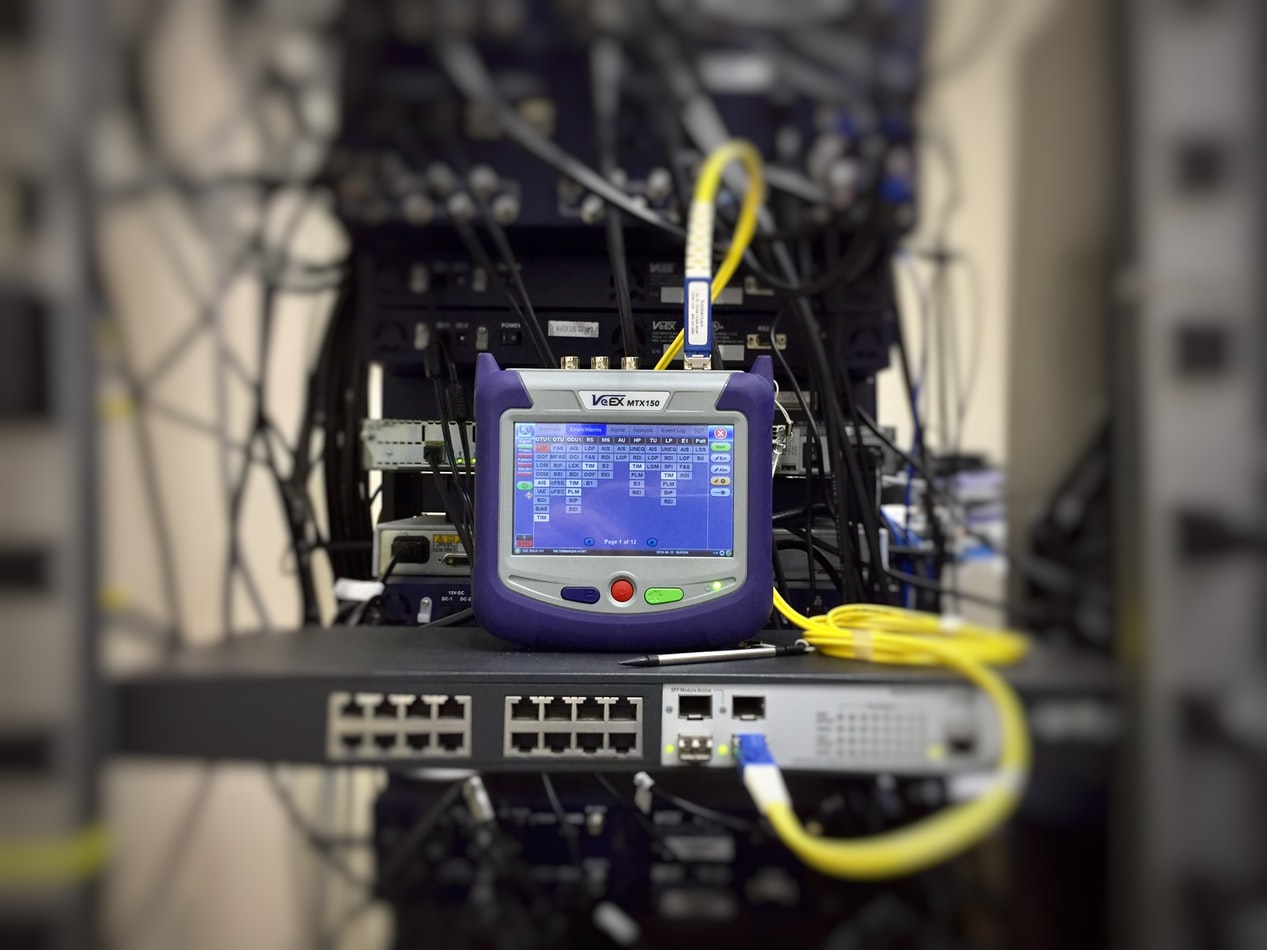
\includegraphics[width=\linewidth]{b}
\end{minipage}
}
\hfill
\subfigure[4]
{
\centering
\begin{minipage}[t]{0.48\linewidth}
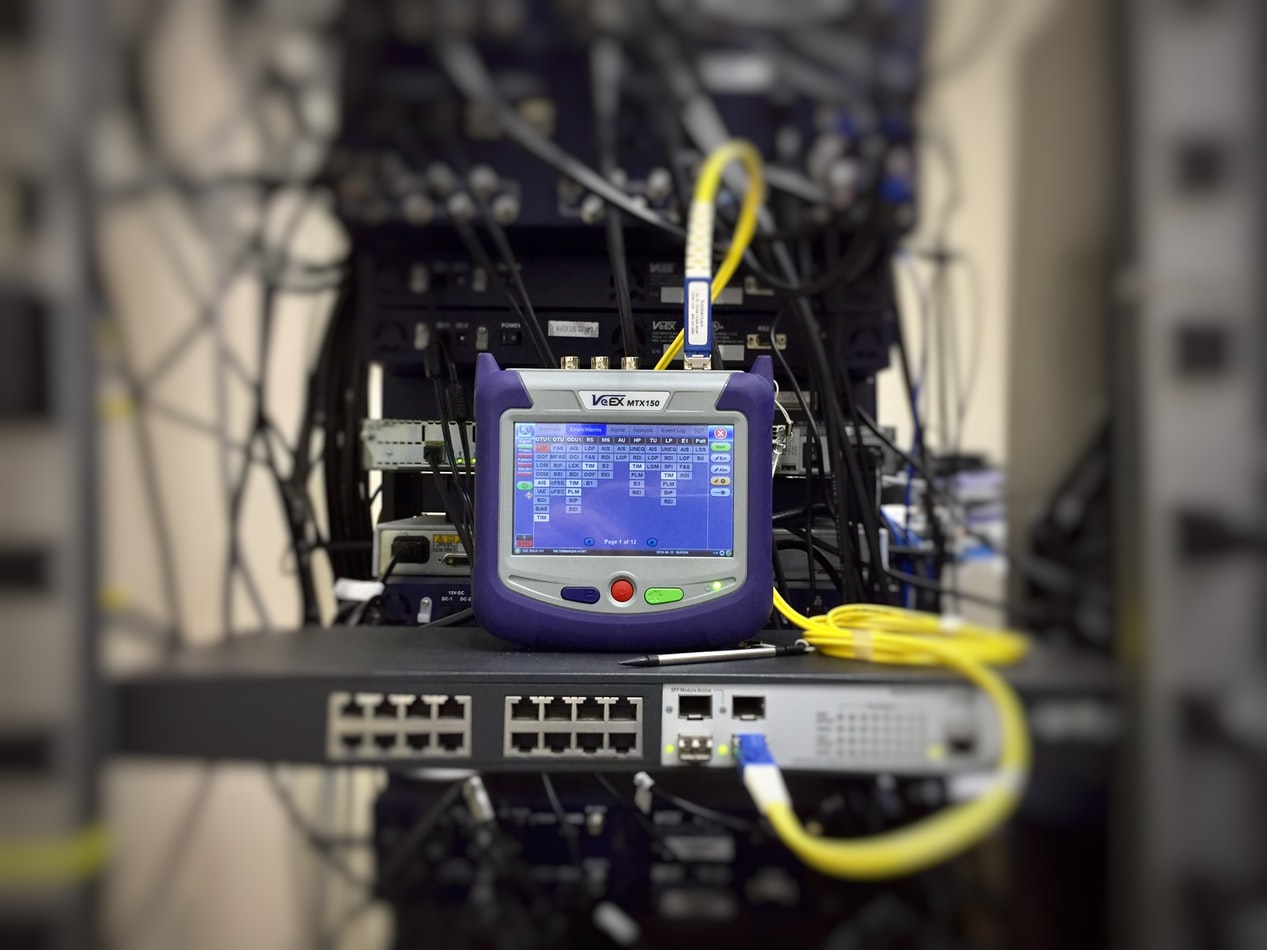
\includegraphics[width=\linewidth]{b}
\end{minipage}
}
\caption{Figure 3} 
\label{fig: 3}  
\end{figure}

\end{lstlisting}

\textbf{The result shows below.}

\begin{figure}[htb]
\centering
\subfigure[1]
{
\centering
\begin{minipage}[t]{0.48\linewidth}

\includegraphics[width=\linewidth]{a}
\end{minipage}
}
\hfill
\subfigure[2]
{
\centering
\begin{minipage}[t]{0.48\linewidth}

\includegraphics[width=\linewidth]{a}
\end{minipage}
}
\\
\subfigure[3]
{
\centering
\begin{minipage}[t]{0.48\linewidth}
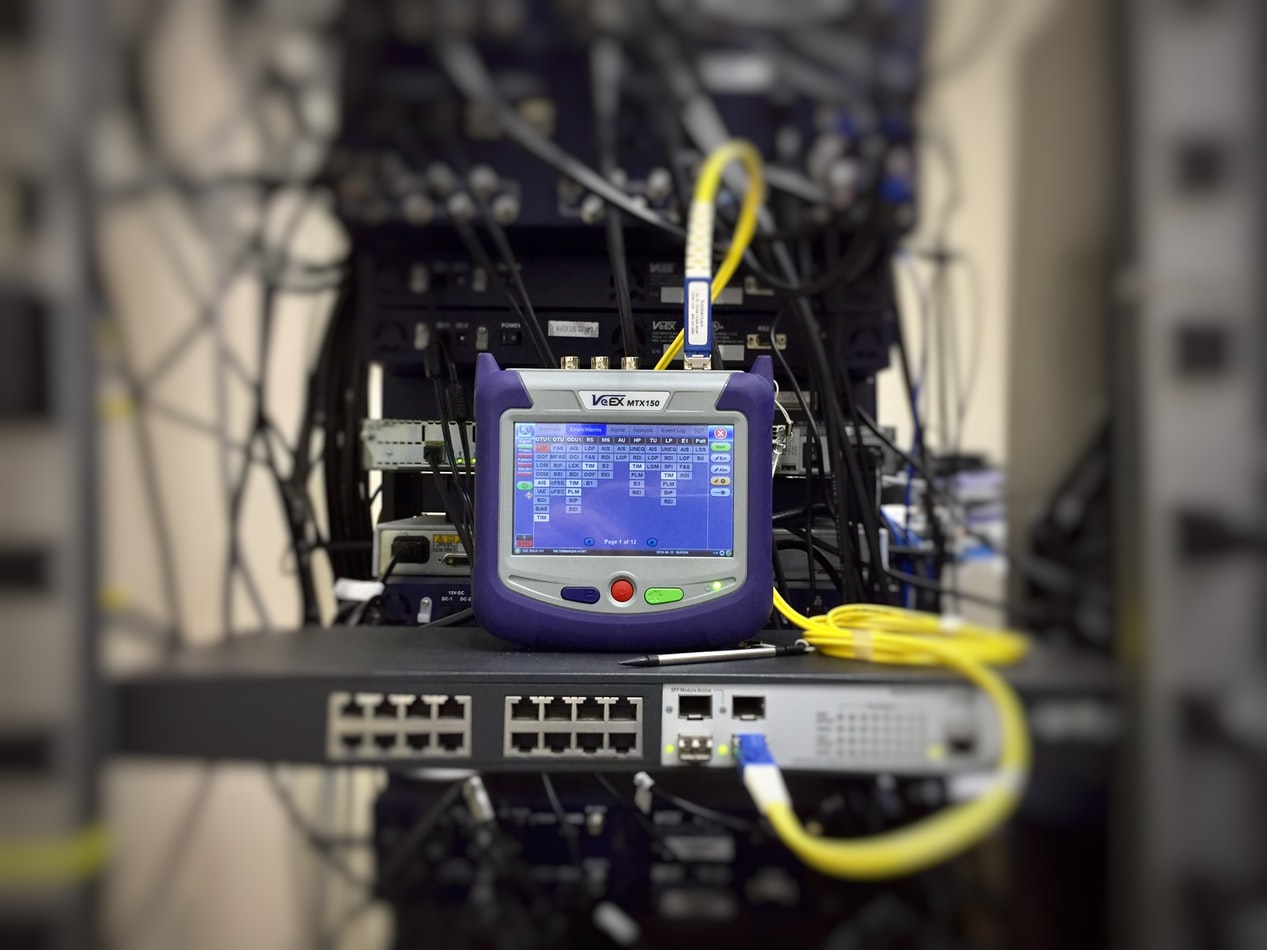
\includegraphics[width=\linewidth]{b}
\end{minipage}
}
\hfill
\subfigure[4]
{
\centering
\begin{minipage}[t]{0.48\linewidth}
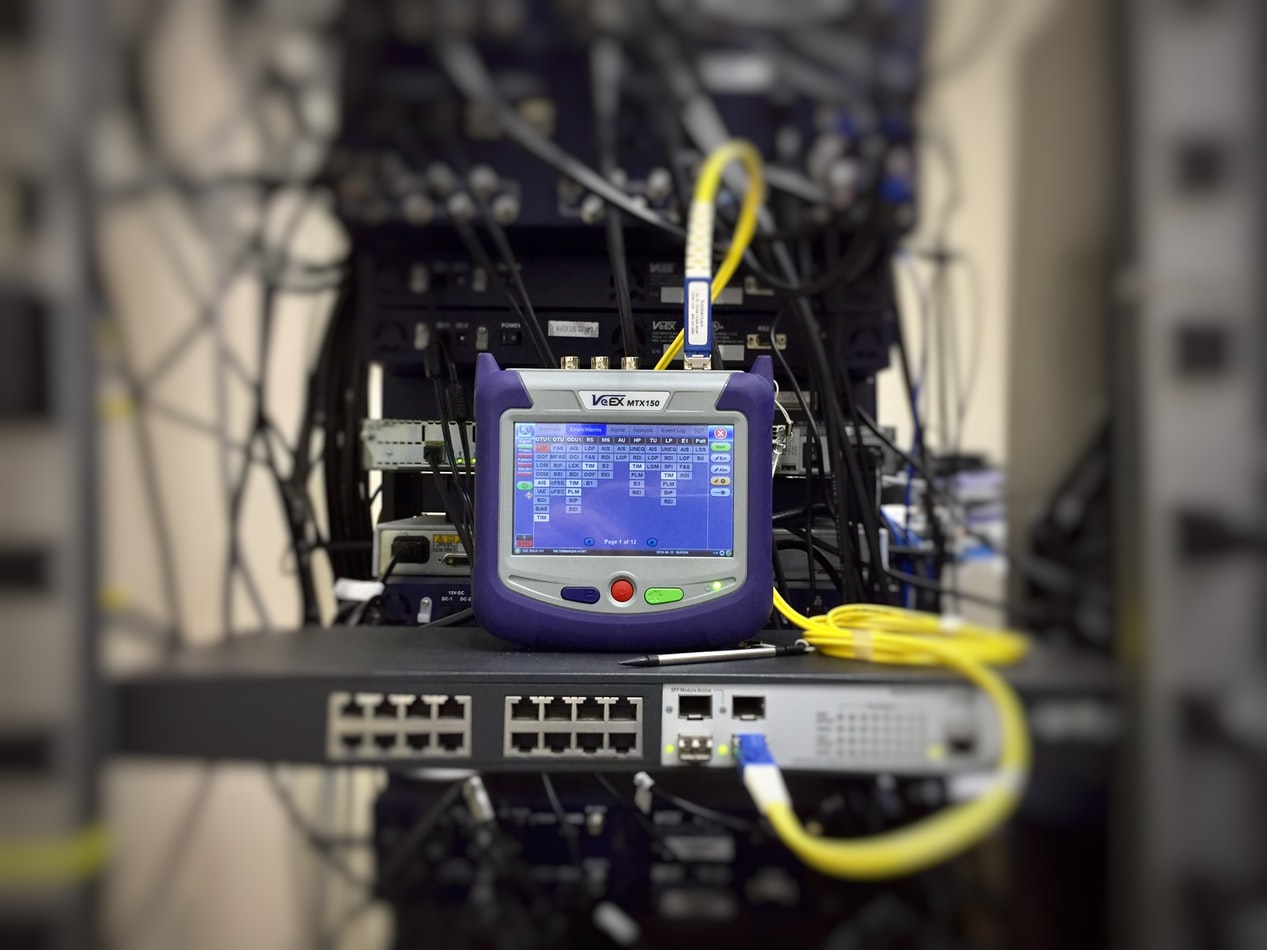
\includegraphics[width=\linewidth]{b}
\end{minipage}
}
\caption{Figure 3} 
\label{fig: 3}  
\end{figure}







%\let\cleardoublepage\clearpage